\begin{IEEEbiography}[{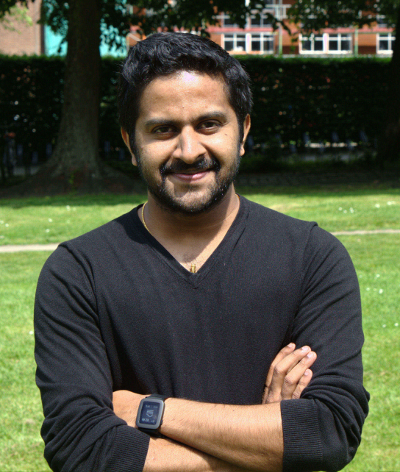
\includegraphics[width=1in,height=1.25in,clip,keepaspectratio]{figures/sreeraj}}]
    {Sreeraj Rajendran}
received his Masters degree in communication and signal processing from the Indian Institute of Technology, Bombay, in 2013. He is currently pursuing the PhD degree in the Department of Electrical Engineering, KU Leuven, Belgium. Before joining KU Leuven, he worked as a senior design engineer in the baseband team of Cadence and as an ASIC verification engineer in Wipro Technologies. His main research interests include machine learning algorithms for wireless and low power wireless sensor networks.
\end{IEEEbiography}

\begin{IEEEbiography}[{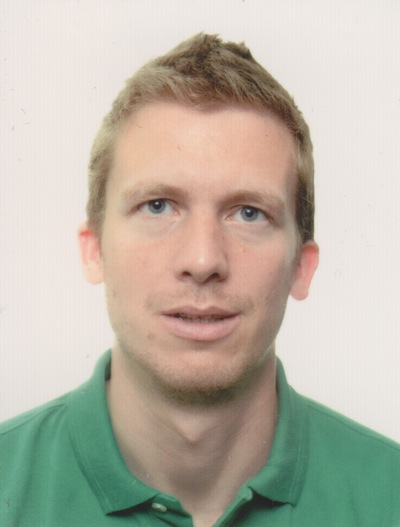
\includegraphics[width=1in,height=1.25in,clip,keepaspectratio]{figures/wannes}}]
    {Wannes Meert}
received his degrees of Master of Electrotechnical Engineering, Micro-electronics (2005), Master of Artificial Intelligence (2006) and Ph.D. in Computer Science (2011) from KU Leuven. He is currently research manager in the DTAI research group at KU Leuven. His work is focused on applying machine learning, artificial intelligence and anomaly detection technology to industrial application domains.
\end{IEEEbiography}

\begin{IEEEbiography}[{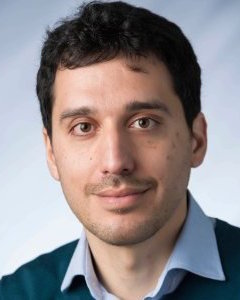
\includegraphics[width=1in,height=1.25in,clip,keepaspectratio]{figures/domenico}}]
    {Domenico Giustiniano}
is Research Associate Professor at IMDEA Networks Institute and leader of the Pervasive Wireless Systems Group. He was formerly a Senior Researcher and Lecturer at ETH Zurich and a Post-
Doctoral Researcher at Disney Research Zurich and at Telefonica Research Barcelona. He holds a Ph.D. from the University of Rome Tor Vergata (2008). He devotes most of his current research to visible light communication, mobile indoor localization, and collaborative spectrum sensing systems. He is an author of more than 70 international papers, leader of the OpenVLC project
and co-founder of the non-profit Electrosense association.
\end{IEEEbiography}

\begin{IEEEbiography}[{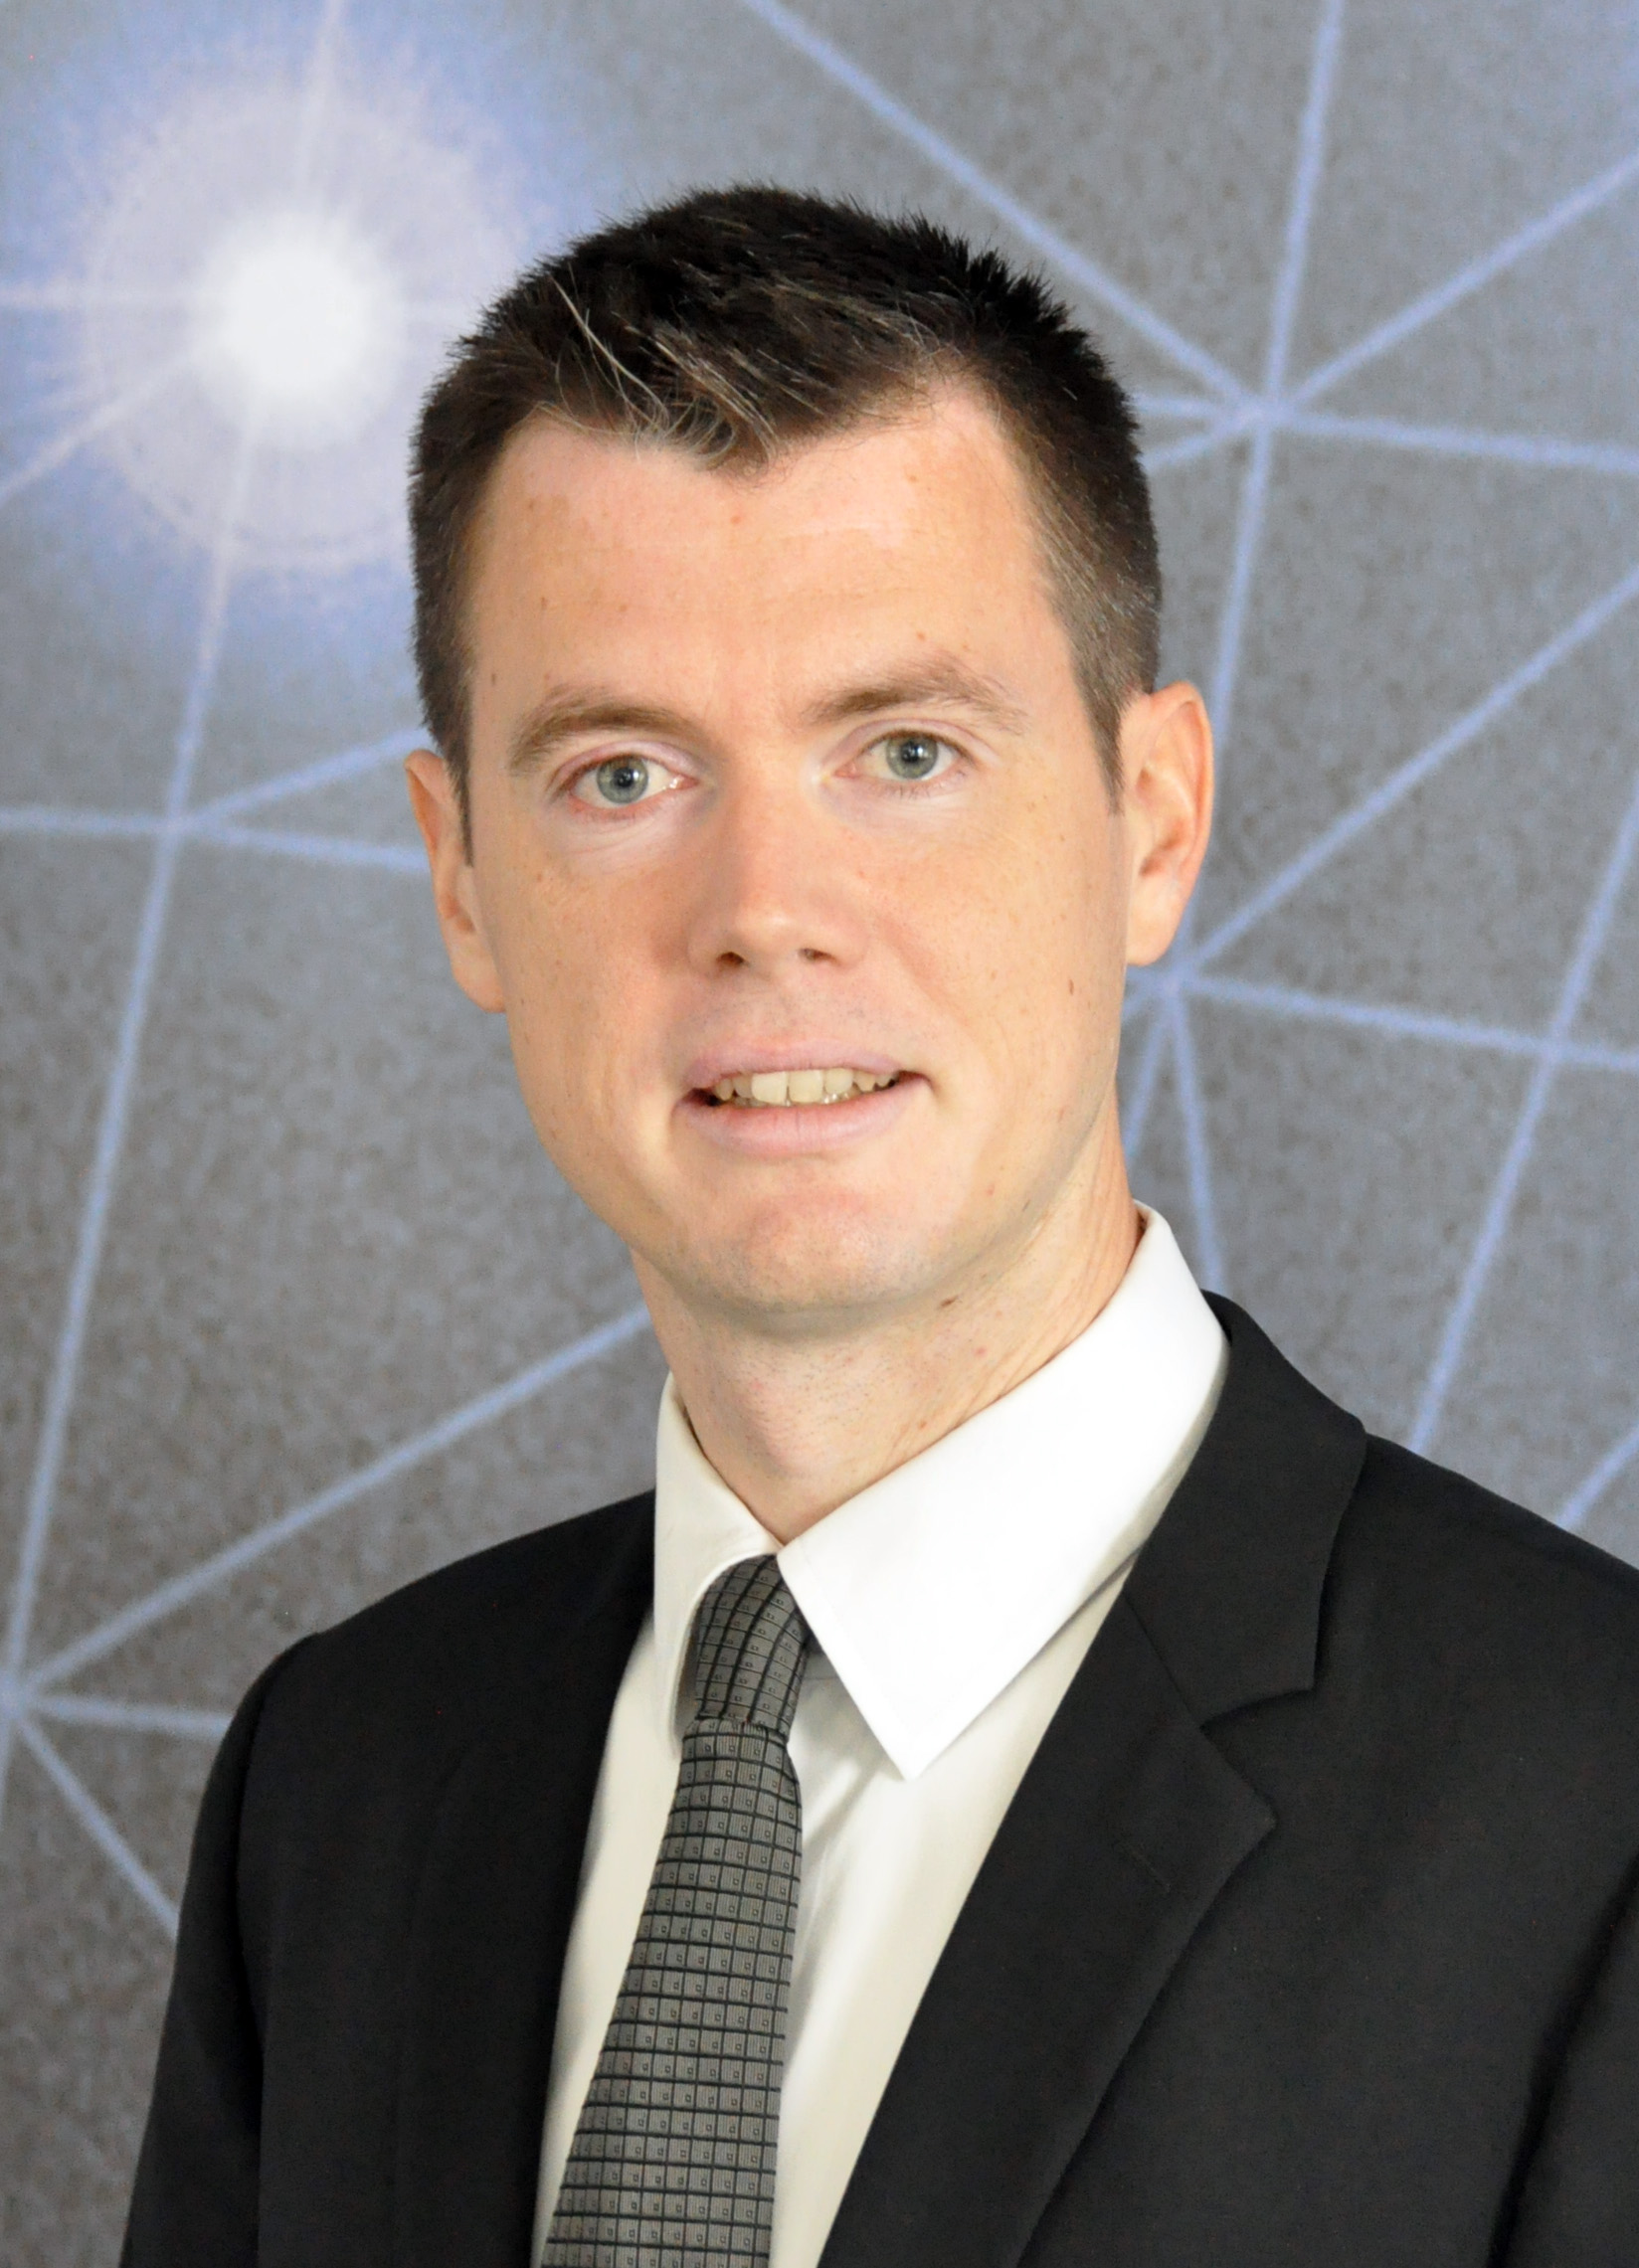
\includegraphics[width=1in,height=1.25in,clip,keepaspectratio]{figures/vincent}}]
    {Vincent Lenders}
is a research director at armasuisse where he leads the cyber and information sciences research of the Swiss Federal Department of Defense. He received the M.Sc. and Ph.D. degrees in electrical engineering from ETH Zurich. He was postdoctoral research fellow at Princeton University. Dr.Vincent Lenders is the cofounder and in the board of the OpenSky Network and Electrosense associations. His current research interests are in the fields of cyber security, information management, big data, and crowdsourcing.
\end{IEEEbiography}

\begin{IEEEbiography}[{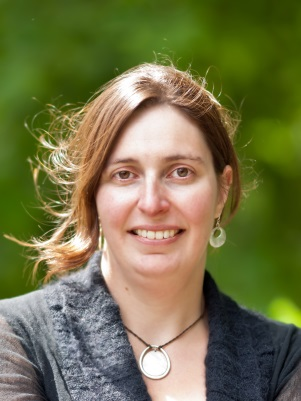
\includegraphics[width=1in,height=1.25in,clip,keepaspectratio]{figures/sofie}}]
    {Sofie Pollin}
obtained her PhD degree at KU Leuven with honors in 2006. From 2006-2008 she continued her research on wireless communication, energy-efficient networks, cross-layer design, coexistence and cognitive radio at UC Berkeley.  In November 2008 she returned to imec to become a principal scientist in the green radio team. Since 2012, she is tenure track assistant professor at the electrical engineering department at KU Leuven. Her research centers around Networked Systems that require networks that are ever more dense, heterogeneous, battery powered and spectrum constrained. Prof. Pollin is BAEF and Marie Curie fellow, and IEEE senior member. 
\end{IEEEbiography}